\documentclass[12pt,letterpaper]{article}
\usepackage[utf8]{inputenc}
\usepackage[spanish]{babel}
\usepackage{graphicx}
\usepackage[left=2cm,right=2cm,top=2cm,bottom=2cm]{geometry}
\usepackage{graphicx} % figuras
\usepackage{hyperref}
% \usepackage{subfigure} % subfiguras
\usepackage{float} % para usar [H]
\usepackage{amsmath}
%\usepackage{txfonts}
\usepackage{stackrel} 
\usepackage{multirow}
\usepackage{enumerate} % enumerados
\renewcommand{\labelitemi}{$-$}
\renewcommand{\labelitemii}{$\cdot$}
% \author{}
% \title{Caratula}
\begin{document}

% Fancy Header and Footer
% \usepackage{fancyhdr}
% \pagestyle{fancy}
% \cfoot{}
% \rfoot{\thepage}
%

% \usepackage[hidelinks]{hyperref} % CREA HYPERVINCULOS EN INDICE

% \author{}
\title{Caratula}

\begin{titlepage}
\begin{center}
\large{UNIVERSIDAD PRIVADA-DE-TACNA}\\
\vspace*{-0.025in}
\begin{figure}[htb]
\begin{center}

\includegraphics[width=8cm]{./Imagenes/logo}
\end{center}
\end{figure}
\vspace*{0.15in}
INGENIERIA DE SISTEMAS  \\

\vspace*{0.5in}
\begin{large}
TITULO:\\
\end{large}

\vspace*{0.1in}
\begin{Large}
\textbf{INFORME DE LABORATORIO Nro 02} \\
\end{Large}

\vspace*{0.3in}
\begin{Large}
\textbf{CURSO:} \\
\end{Large}

\vspace*{0.1in}
\begin{large}
INTELIGENCIA DE NEGOCIOS\\
\end{large}

\vspace*{0.3in}
\begin{Large}
\textbf{DOCENTE(ING):} \\
\end{Large}

\vspace*{0.1in}
\begin{large}
 Patrick Cuadros Quiroga\\
\end{large}

\vspace*{0.2in}
\vspace*{0.1in}
\begin{large}
Integrante: \\
\begin{flushleft}
Marlon Xavier Villegas Arando	\hfill	(2015053890) 
\end{flushleft}
\end{large}
\end{center}

\end{titlepage}



\thispagestyle{empty} % INDICE SIN NUMERO
\newpage
\setcounter{page}{1} % REINICIAR CONTADOR DE PAGINAS DESPUES DEL INDICE

\section{INFORMACIÓN GENERAL}
	\begin{itemize}
\subsection{Objetivos:}
	\item Realizar relaciones de tablas con PowerBI
	\item Aprender a elaborar tablas de reportes combinando resultados de columnas para generar nuevos datos.
\subsection{Equipos, materiales, programas y recursos utilizados:}
	\item Microsoft SQL Server 2017 o SQL Lite
	\item Base de datos AdventureWorks2017
	\item Power Bi Desktop
\end{itemize}

\section{MARCO TEORICO}
\begin{itemize}
\subsection{Power Bi:}
	\item Solución de análisis empresarial que permite visualizar datos y compartir información de toda una organización, o insertarla en su aplicación o sitio web. 
\subsection{Dashboard:}
	\item Presenta el contenido de una serie de indicadores que muestran el comportamiento de los datos. 
\end{itemize}
\section{PROCEDIMIENTO}
\begin{itemize}
	\item \textbf{Tarea 1:} Crear Realiciones 
	\item Iniciar Power Bi Desktop; click en Obtener Datos , click en Excel el archivo Adventure Works Sales Data.xlsx y abrir
	\item  Seleccionar las hojas DimCurrency, DimCustomer, DimDate, DimProduct, DimPromotion, DimSalesTerritory y FactInternetSales
	\item \textbf{Tarea 2:} Relaciones Manuales
	\item Relacionar las tablas DimProductCategory y DimProductSubcategory en la pestaña de relaciones
	\item \textbf{Tarea 3:} Cálculos
	\item agregar una nueva columna y escribir en la barra de formula en la tabla de DimCustomer Column = IncomeStatus = IF (DimCustomer[YearlyIncome] < 25000, "Lower Income",
IF (AND(DimCustomer[YearlyIncome] >= 25000, DimCustomer[YearlyIncome] < 60000),
"Middle Income",
IF (AND(DimCustomer[YearlyIncome] >= 60000, DimCustomer[YearlyIncome] < 100000),
"Higher Income",
IF (DimCustomer[YearlyIncome] >= 100000, "Very High Income", "Other"))))
\end{itemize}
\section{ANALISIS E INTERPRETACIÓN DE DATOS}

	\begin{center}
	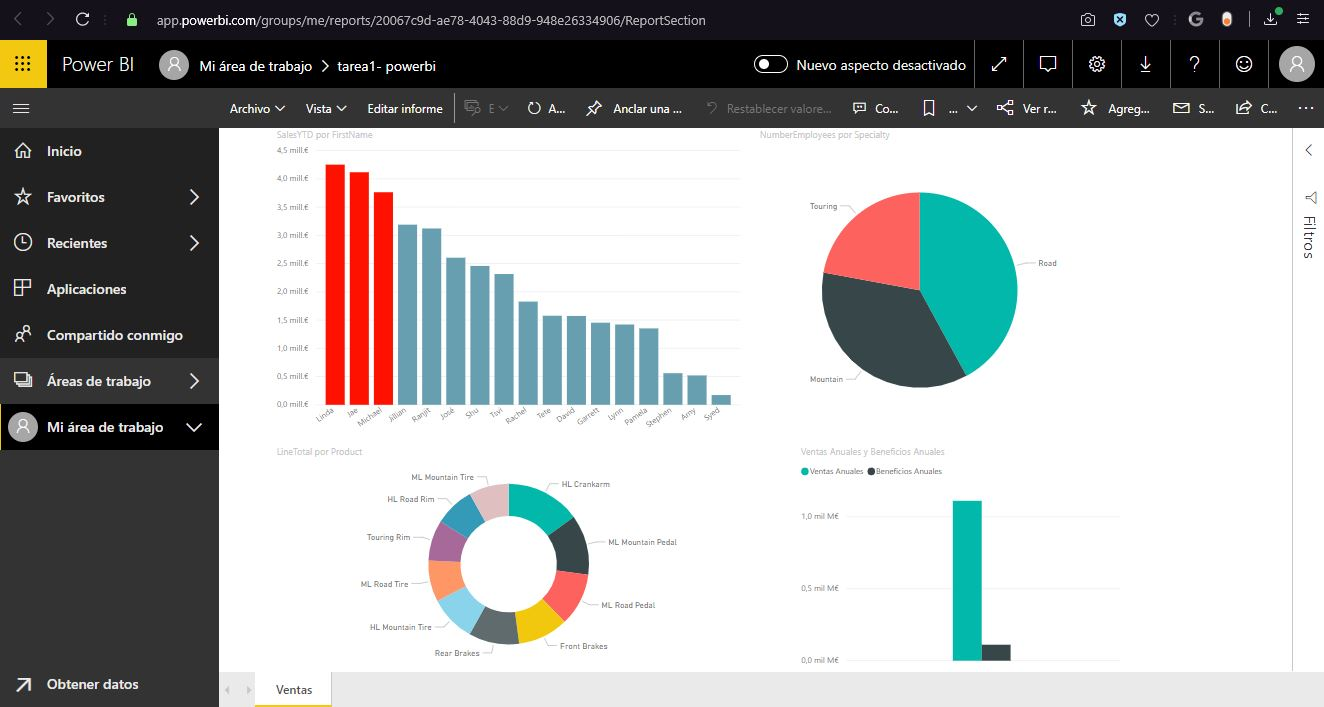
\includegraphics[width=16cm]{./Imagenes/img}
	\end{center}
	\begin{center}
	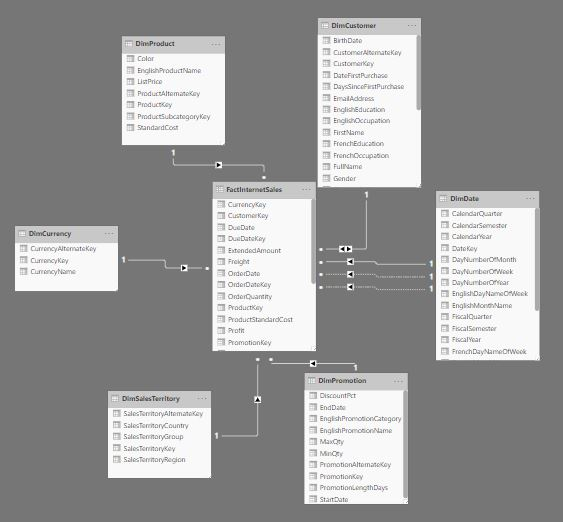
\includegraphics[width=16cm]{./Imagenes/img2}
	\end{center}
	\begin{center}
	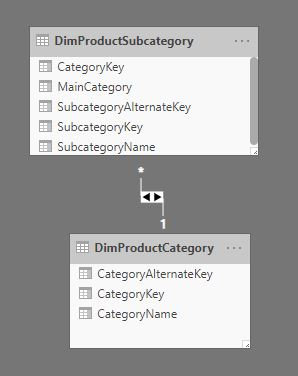
\includegraphics[width=16cm]{./Imagenes/img3}
	\end{center}
	\begin{center}
	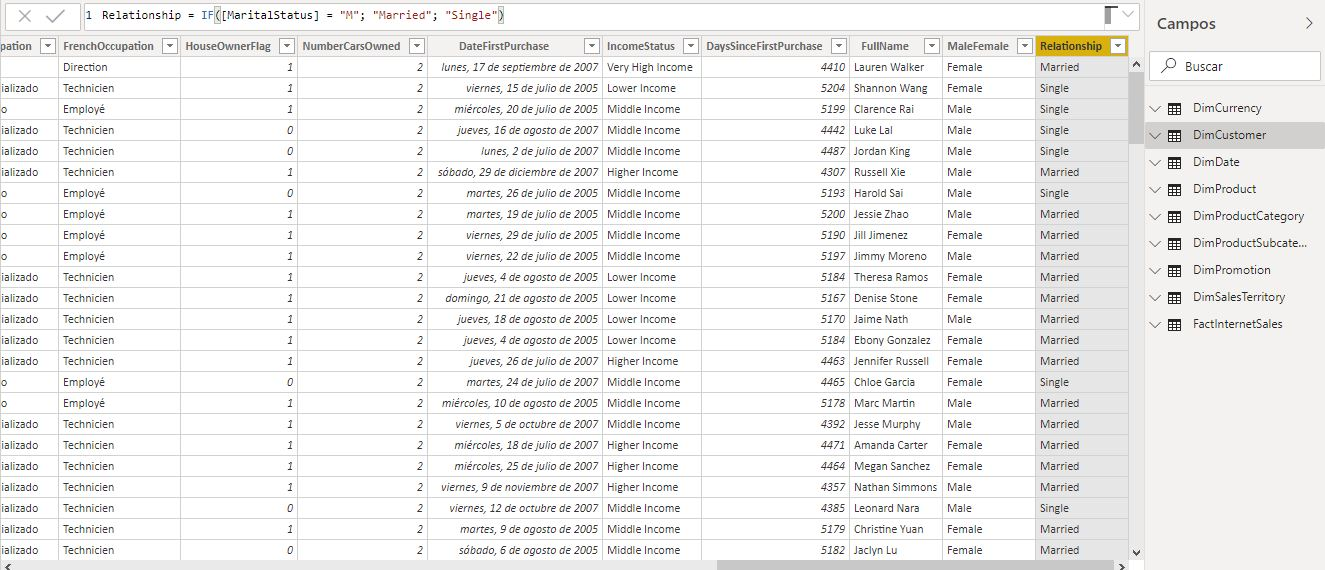
\includegraphics[width=16cm]{./Imagenes/img4}
	\end{center}
\par https://app.powerbi.com/groups/me/reports/6baf1255-f121-4c3f-be26-3a324c76c1c4/ReportSection
\section{CONCLUSIONES}
\begin{itemize}
	\item En el desarrollo del laboratorio nos enseña que podemos importar datos desde archivos excel.
	\item Podemos crear relaciones en base a datos de excel y realizar columnas funcion para simplificar la informacion y obtener los datos requeridos.
\end{itemize}
\section{REFERENCIAS}
\begin{itemize}
	\item Microsoft. ¿Qué es Power BI?. Recuperado de \url{https://powerbi.microsoft.com/es-es/what-is-power-bi/}
	\item Jortilles. Crear un dashboard con Pentaho Bi-Server. Recuperado de \url{http://www.jortilles.com/wp-content/uploads/2016/04/DashboardCDE_Pentaho.pdf}

\end{itemize}


\end{document}
